\documentclass{report}
\usepackage[english]{babel}

%%%%%%%%%%%%%%%%%%%%%%%%%%%%%%%%%
% PACKAGE IMPORTS
%%%%%%%%%%%%%%%%%%%%%%%%%%%%%%%%%


\usepackage[tmargin=2cm,rmargin=1in,lmargin=1in,margin=0.85in,bmargin=2cm,footskip=.2in]{geometry}
\usepackage{amsmath,amsfonts,amsthm,amssymb,mathtools}
\usepackage{wrapfig}
\usepackage{subcaption}
\usepackage{afterpage}
\usepackage[varbb]{newpxmath}
\usepackage{xfrac}
\usepackage[T1]{fontenc}
\usepackage{tabularx}
\usepackage{floatrow}
\usepackage{enumerate}
\newfloatcommand{capbtabbox}{table}[][\FBwidth]
\usepackage{amssymb}
%command for alg-closure that automatically adapts its 'bar' to the arg based on the args length (including '\')
\newcommand{\ols}[1]{\mskip.5\thinmuskip\overline{\mskip-.5\thinmuskip {#1} \mskip-.5\thinmuskip}\mskip.5\thinmuskip} % overline short
\newcommand{\olsi}[1]{\,\overline{\!{#1}}} % overline short italic
\makeatletter
\newcommand\ovl[1]{
  \tctestifnum{\count@stringtoks{#1}>1} %checks if number of chars in arg > 1 (including '\')
  {\ols{#1}} %if arg is longer than just one char, e.g. \mathbb{Q}, \mathbb{F},...
  {\olsi{#1}} %if arg is just one char, e.g. K, L,...
}
% FROM TOKCYCLE:
\long\def\count@stringtoks#1{\tc@earg\count@toks{\string#1}}
\long\def\count@toks#1{\the\numexpr-1\count@@toks#1.\tc@endcnt}
\long\def\count@@toks#1#2\tc@endcnt{+1\tc@ifempty{#2}{\relax}{\count@@toks#2\tc@endcnt}}
\def\tc@ifempty#1{\tc@testxifx{\expandafter\relax\detokenize{#1}\relax}}
\long\def\tc@earg#1#2{\expandafter#1\expandafter{#2}}
\long\def\tctestifnum#1{\tctestifcon{\ifnum#1\relax}}
\long\def\tctestifcon#1{#1\expandafter\tc@exfirst\else\expandafter\tc@exsecond\fi}
\long\def\tc@testxifx{\tc@earg\tctestifx}
\long\def\tctestifx#1{\tctestifcon{\ifx#1}}
\long\def\tc@exfirst#1#2{#1}
\long\def\tc@exsecond#1#2{#2}
\makeatother
\usepackage[makeroom]{cancel}
\usepackage{mathtools}
\usepackage{bookmark}
\usepackage{enumitem}
\usepackage{hyperref,theoremref}
\hypersetup{
	pdftitle={Apuntes de Análisis de Varias Variables 2},
	colorlinks=true, linkcolor=doc!90,
	bookmarksnumbered=true,
	bookmarksopen=true
}
\usepackage[most,many,breakable]{tcolorbox}
\usepackage{xcolor}
\usepackage{varwidth}
\usepackage{varwidth}
\usepackage{etoolbox}
%\usepackage{authblk}
\usepackage{nameref}
\usepackage{multicol,array}
\usepackage{tikz-cd}
\usepackage[ruled,vlined,linesnumbered]{algorithm2e}
\usepackage{comment} % enables the use of multi-line comments (\ifx \fi) 
\usepackage{import}
\usepackage{xifthen}
\usepackage{pdfpages}
\usepackage{transparent}
\usepackage{titlesec}
\titleformat{\section}{\normalfont\fontsize{17.28pt}{12pt}\selectfont\bfseries}{\thesection}{1em}{}
\usepackage{empheq} % boxed align


\newcommand\mycommfont[1]{\footnotesize\ttfamily\textcolor{blue}{#1}}
\SetCommentSty{mycommfont}
\newcommand{\incfig}[1]{%
    \def\svgwidth{\columnwidth}
    \import{./figures/}{#1.pdf_tex}
}

\newcommand{\notimplies}{\;\not\!\!\!\implies}

\usepackage{tikzsymbols}
\renewcommand\qedsymbol{$\Laughey$}

\newcommand\phantomarrow[2]{%
  \setbox0=\hbox{$\displaystyle #1\to$}%
  \hbox to \wd0{%
    $#2\mapstochar
     \cleaders\hbox{$\mkern-1mu\relbar\mkern-3mu$}\hfill
     \mkern-7mu\rightarrow$}%
  \,}

%\usepackage{import}
%\usepackage{xifthen}
%\usepackage{pdfpages}
%\usepackage{transparent}


%%%%%%%%%%%%%%%%%%%%%%%%%%%%%%
% SELF MADE COLORS
%%%%%%%%%%%%%%%%%%%%%%%%%%%%%%



\definecolor{myg}{RGB}{56, 140, 70}
\definecolor{myb}{RGB}{45, 111, 177}
\definecolor{myr}{RGB}{199, 68, 64}
\definecolor{mytheorembg}{HTML}{f5e4e1}
\definecolor{mytheoremfr}{HTML}{7B0000}
\definecolor{mylenmabg}{HTML}{FFFAF8}
\definecolor{mylenmafr}{HTML}{983b0f}
\definecolor{mypropbg}{HTML}{f2fbfc}
\definecolor{mypropfr}{HTML}{191971}
\definecolor{myexamplebg}{HTML}{F2FBF8}
\definecolor{myexamplefr}{HTML}{88D6D1}
\definecolor{myexampleti}{HTML}{2A7F7F}
\definecolor{mydefinitbg}{HTML}{E5E5FF}
\definecolor{mydefinitfr}{HTML}{3F3FA3}
\definecolor{notesgreen}{RGB}{0,162,0}
\definecolor{myp}{RGB}{197, 92, 212}
\definecolor{mygr}{HTML}{2C3338}
\definecolor{myred}{RGB}{127,0,0}
\definecolor{myyellow}{RGB}{169,121,69}
\definecolor{myexercisebg}{HTML}{F2FBF8}
\definecolor{myexercisefg}{HTML}{2A7F7F}


%%%%%%%%%%%%%%%%%%%%%%%%%%%%
% TCOLORBOX SETUPS
%%%%%%%%%%%%%%%%%%%%%%%%%%%%

\setlength{\parindent}{1cm}
%================================
% THEOREM BOX
%================================

\tcbuselibrary{theorems,skins,hooks}
\newtcbtheorem[number within=section]{Theorem}{Teorema}
{%
	enhanced,
	breakable,
	colback = mytheorembg,
	frame hidden,
	boxrule = 0sp,
	borderline west = {2pt}{0pt}{mytheoremfr},
	sharp corners,
	detach title,
	before upper = \tcbtitle\par\smallskip,
	coltitle = mytheoremfr,
	fonttitle = \bfseries\sffamily,
	description font = \mdseries,
	separator sign none,
	segmentation style={solid, mytheoremfr},
}
{th}

\tcbuselibrary{theorems,skins,hooks}
\newtcbtheorem[number within=chapter]{theorem}{Teorema}
{%
	enhanced,
	breakable,
	colback = mytheorembg,
	frame hidden,
	boxrule = 0sp,
	borderline west = {2pt}{0pt}{mytheoremfr},
	sharp corners,
	detach title,
	before upper = \tcbtitle\par\smallskip,
	coltitle = mytheoremfr,
	fonttitle = \bfseries\sffamily,
	description font = \mdseries,
	separator sign none,
	segmentation style={solid, mytheoremfr},
}
{th}


\tcbuselibrary{theorems,skins,hooks}
\newtcolorbox{Theoremcon}
{%
	enhanced
	,breakable
	,colback = mytheorembg
	,frame hidden
	,boxrule = 0sp
	,borderline west = {2pt}{0pt}{mytheoremfr}
	,sharp corners
	,description font = \mdseries
	,separator sign none
}

%================================
% Corollary
%================================
\tcbuselibrary{theorems,skins,hooks}
\newtcbtheorem[number within=section]{Corollary}{Corolario}
{%
	enhanced
	,breakable
	,colback = myp!10
	,frame hidden
	,boxrule = 0sp
	,borderline west = {2pt}{0pt}{myp!85!black}
	,sharp corners
	,detach title
	,before upper = \tcbtitle\par\smallskip
	,coltitle = myp!85!black
	,fonttitle = \bfseries\sffamily
	,description font = \mdseries
	,separator sign none
	,segmentation style={solid, myp!85!black}
}
{th}
\tcbuselibrary{theorems,skins,hooks}
\newtcbtheorem[number within=chapter]{corollary}{Corolario}
{%
	enhanced
	,breakable
	,colback = myp!10
	,frame hidden
	,boxrule = 0sp
	,borderline west = {2pt}{0pt}{myp!85!black}
	,sharp corners
	,detach title
	,before upper = \tcbtitle\par\smallskip
	,coltitle = myp!85!black
	,fonttitle = \bfseries\sffamily
	,description font = \mdseries
	,separator sign none
	,segmentation style={solid, myp!85!black}
}
{th}


%================================
% LENMA
%================================

\tcbuselibrary{theorems,skins,hooks}
\newtcbtheorem[number within=section]{Lenma}{Lenma}
{%
	enhanced,
	breakable,
	colback = mylenmabg,
	frame hidden,
	boxrule = 0sp,
	borderline west = {2pt}{0pt}{mylenmafr},
	sharp corners,
	detach title,
	before upper = \tcbtitle\par\smallskip,
	coltitle = mylenmafr,
	fonttitle = \bfseries\sffamily,
	description font = \mdseries,
	separator sign none,
	segmentation style={solid, mylenmafr},
}
{th}

\tcbuselibrary{theorems,skins,hooks}
\newtcbtheorem[number within=chapter]{lenma}{Lenma}
{%
	enhanced,
	breakable,
	colback = mylenmabg,
	frame hidden,
	boxrule = 0sp,
	borderline west = {2pt}{0pt}{mylenmafr},
	sharp corners,
	detach title,
	before upper = \tcbtitle\par\smallskip,
	coltitle = mylenmafr,
	fonttitle = \bfseries\sffamily,
	description font = \mdseries,
	separator sign none,
	segmentation style={solid, mylenmafr},
}
{th}


%================================
% PROPOSITION
%================================

\tcbuselibrary{theorems,skins,hooks}
\newtcbtheorem[number within=section]{Prop}{Proposition}
{%
	enhanced,
	breakable,
	colback = mypropbg,
	frame hidden,
	boxrule = 0sp,
	borderline west = {2pt}{0pt}{mypropfr},
	sharp corners,
	detach title,
	before upper = \tcbtitle\par\smallskip,
	coltitle = mypropfr,
	fonttitle = \bfseries\sffamily,
	description font = \mdseries,
	separator sign none,
	segmentation style={solid, mypropfr},
}
{th}

\tcbuselibrary{theorems,skins,hooks}
\newtcbtheorem[number within=chapter]{prop}{Proposition}
{%
	enhanced,
	breakable,
	colback = mypropbg,
	frame hidden,
	boxrule = 0sp,
	borderline west = {2pt}{0pt}{mypropfr},
	sharp corners,
	detach title,
	before upper = \tcbtitle\par\smallskip,
	coltitle = mypropfr,
	fonttitle = \bfseries\sffamily,
	description font = \mdseries,
	separator sign none,
	segmentation style={solid, mypropfr},
}
{th}


%================================
% CLAIM
%================================

\tcbuselibrary{theorems,skins,hooks}
\newtcbtheorem[number within=section]{claim}{Claim}
{%
	enhanced
	,breakable
	,colback = myg!10
	,frame hidden
	,boxrule = 0sp
	,borderline west = {2pt}{0pt}{myg}
	,sharp corners
	,detach title
	,before upper = \tcbtitle\par\smallskip
	,coltitle = myg!85!black
	,fonttitle = \bfseries\sffamily
	,description font = \mdseries
	,separator sign none
	,segmentation style={solid, myg!85!black}
}
{th}



%================================
% Exercise
%================================

\tcbuselibrary{theorems,skins,hooks}
\newtcbtheorem[number within=section]{Exercise}{Ejercicio}
{%
	enhanced,
	breakable,
	colback = myexercisebg,
	frame hidden,
	boxrule = 0sp,
	borderline west = {2pt}{0pt}{myexercisefg},
	sharp corners,
	detach title,
	before upper = \tcbtitle\par\smallskip,
	coltitle = myexercisefg,
	fonttitle = \bfseries\sffamily,
	description font = \mdseries,
	separator sign none,
	segmentation style={solid, myexercisefg},
}
{th}

\tcbuselibrary{theorems,skins,hooks}
\newtcbtheorem[number within=chapter]{exercise}{Ejercicio}
{%
	enhanced,
	breakable,
	colback = myexercisebg,
	frame hidden,
	boxrule = 0sp,
	borderline west = {2pt}{0pt}{myexercisefg},
	sharp corners,
	detach title,
	before upper = \tcbtitle\par\smallskip,
	coltitle = myexercisefg,
	fonttitle = \bfseries\sffamily,
	description font = \mdseries,
	separator sign none,
	segmentation style={solid, myexercisefg},
}
{th}

%================================
% EXAMPLE BOX
%================================

\newtcbtheorem[number within=section]{Example}{Ejemplo}
{%
	colback = myexamplebg
	,breakable
	,colframe = myexamplefr
	,coltitle = myexampleti
	,boxrule = 1pt
	,sharp corners
	,detach title
	,before upper=\tcbtitle\par\smallskip
	,fonttitle = \bfseries
	,description font = \mdseries
	,separator sign none
	,description delimiters parenthesis
}
{ex}

\newtcbtheorem[number within=chapter]{example}{Ejemplo}
{%
	colback = myexamplebg
	,breakable
	,colframe = myexamplefr
	,coltitle = myexampleti
	,boxrule = 1pt
	,sharp corners
	,detach title
	,before upper=\tcbtitle\par\smallskip
	,fonttitle = \bfseries
	,description font = \mdseries
	,separator sign none
	,description delimiters parenthesis
}
{ex}

%================================
% DEFINITION BOX
%================================

\newtcbtheorem[number within=section]{Definition}{Definición}{enhanced,
	before skip=2mm,after skip=2mm, colback=blue!5,colframe=blue!80!black,boxrule=0.5mm,
	attach boxed title to top left={xshift=1cm,yshift*=1mm-\tcboxedtitleheight}, varwidth boxed title*=-3cm,
	boxed title style={frame code={
					\path[fill=tcbcolback]
					([yshift=-1mm,xshift=-1mm]frame.north west)
					arc[start angle=0,end angle=180,radius=1mm]
					([yshift=-1mm,xshift=1mm]frame.north east)
					arc[start angle=180,end angle=0,radius=1mm];
					\path[left color=tcbcolback!60!black,right color=tcbcolback!60!black,
						middle color=tcbcolback!80!black]
					([xshift=-2mm]frame.north west) -- ([xshift=2mm]frame.north east)
					[rounded corners=1mm]-- ([xshift=1mm,yshift=-1mm]frame.north east)
					-- (frame.south east) -- (frame.south west)
					-- ([xshift=-1mm,yshift=-1mm]frame.north west)
					[sharp corners]-- cycle;
				},interior engine=empty,
		},
	fonttitle=\bfseries,
	title={#2},#1}{def}
\newtcbtheorem[number within=chapter]{definition}{Definición}{enhanced,
	before skip=2mm,after skip=2mm, colback=red!5,colframe=red!80!black,boxrule=0.5mm,
	attach boxed title to top left={xshift=1cm,yshift*=1mm-\tcboxedtitleheight}, varwidth boxed title*=-3cm,
	boxed title style={frame code={
					\path[fill=tcbcolback]
					([yshift=-1mm,xshift=-1mm]frame.north west)
					arc[start angle=0,end angle=180,radius=1mm]
					([yshift=-1mm,xshift=1mm]frame.north east)
					arc[start angle=180,end angle=0,radius=1mm];
					\path[left color=tcbcolback!60!black,right color=tcbcolback!60!black,
						middle color=tcbcolback!80!black]
					([xshift=-2mm]frame.north west) -- ([xshift=2mm]frame.north east)
					[rounded corners=1mm]-- ([xshift=1mm,yshift=-1mm]frame.north east)
					-- (frame.south east) -- (frame.south west)
					-- ([xshift=-1mm,yshift=-1mm]frame.north west)
					[sharp corners]-- cycle;
				},interior engine=empty,
		},
	fonttitle=\bfseries,
	title={#2},#1}{def}



%================================
% Solution BOX
%================================

\makeatletter
\newtcbtheorem{question}{Cuestión}{enhanced,
	breakable,
	colback=white,
	colframe=myb!80!black,
	attach boxed title to top left={yshift*=-\tcboxedtitleheight},
	fonttitle=\bfseries,
	title={#2},
	boxed title size=title,
	boxed title style={%
			sharp corners,
			rounded corners=northwest,
			colback=tcbcolframe,
			boxrule=0pt,
		},
	underlay boxed title={%
			\path[fill=tcbcolframe] (title.south west)--(title.south east)
			to[out=0, in=180] ([xshift=5mm]title.east)--
			(title.center-|frame.east)
			[rounded corners=\kvtcb@arc] |-
			(frame.north) -| cycle;
		},
	#1
}{def}
\makeatother

%================================
% SOLUTION BOX
%================================

\makeatletter
\newtcolorbox{solution}{enhanced,
	breakable,
	colback=white,
	colframe=myg!80!black,
	attach boxed title to top left={yshift*=-\tcboxedtitleheight},
	title=Solution,
	boxed title size=title,
	boxed title style={%
			sharp corners,
			rounded corners=northwest,
			colback=tcbcolframe,
			boxrule=0pt,
		},
	underlay boxed title={%
			\path[fill=tcbcolframe] (title.south west)--(title.south east)
			to[out=0, in=180] ([xshift=5mm]title.east)--
			(title.center-|frame.east)
			[rounded corners=\kvtcb@arc] |-
			(frame.north) -| cycle;
		},
}
\makeatother

%================================
% Question BOX
%================================

\makeatletter
\newtcbtheorem{qstion}{Cuestión}{enhanced,
	breakable,
	colback=white,
	colframe=mygr,
	attach boxed title to top left={yshift*=-\tcboxedtitleheight},
	fonttitle=\bfseries,
	title={#2},
	boxed title size=title,
	boxed title style={%
			sharp corners,
			rounded corners=northwest,
			colback=tcbcolframe,
			boxrule=0pt,
		},
	underlay boxed title={%
			\path[fill=tcbcolframe] (title.south west)--(title.south east)
			to[out=0, in=180] ([xshift=5mm]title.east)--
			(title.center-|frame.east)
			[rounded corners=\kvtcb@arc] |-
			(frame.north) -| cycle;
		},
	#1
}{def}
\makeatother

\newtcbtheorem[number within=chapter]{wconc}{Wrong Concept}{
	breakable,
	enhanced,
	colback=white,
	colframe=myr,
	arc=0pt,
	outer arc=0pt,
	fonttitle=\bfseries\sffamily\large,
	colbacktitle=myr,
	attach boxed title to top left={},
	boxed title style={
			enhanced,
			skin=enhancedfirst jigsaw,
			arc=3pt,
			bottom=0pt,
			interior style={fill=myr}
		},
	#1
}{def}



%================================
% NOTE BOX
%================================

\usetikzlibrary{arrows,calc,shadows.blur}
\tcbuselibrary{skins}
\newtcolorbox{note}[1][]{%
	enhanced jigsaw,
	colback=gray!10!white,%
	colframe=gray!80!black,
	size=small,
	boxrule=1pt,
	title=\textbf{Comentario:},
	halign title=flush center,
	coltitle=black,
	breakable,
	drop shadow=black!50!white,
	attach boxed title to top left={xshift=1cm,yshift=-\tcboxedtitleheight/2,yshifttext=-\tcboxedtitleheight/2},
	minipage boxed title=2.5cm,
	boxed title style={%
			colback=white,
			size=fbox,
			boxrule=1pt,
			boxsep=2pt,
			underlay={%
					\coordinate (dotA) at ($(interior.west) + (-0.5pt,0)$);
					\coordinate (dotB) at ($(interior.east) + (0.5pt,0)$);
					\begin{scope}
						\clip (interior.north west) rectangle ([xshift=3ex]interior.east);
						\filldraw [white, blur shadow={shadow opacity=60, shadow yshift=-.75ex}, rounded corners=2pt] (interior.north west) rectangle (interior.south east);
					\end{scope}
					\begin{scope}[gray!80!black]
						\fill (dotA) circle (2pt);
						\fill (dotB) circle (2pt);
					\end{scope}
				},
		},
	#1,
}

%%%%%%%%%%%%%%%%%%%%%%%%%%%%%%
% SELF MADE COMMANDS
%%%%%%%%%%%%%%%%%%%%%%%%%%%%%%

\newcommand{\ejercicio}[2]{\begin{Exercise}{#1}{}#2\end{Exercise}}
\newcommand{\corolario}[2]{\begin{Corollary}{#1}{}#2\end{Corollary}}
\newcommand{\teorema}[2]{\begin{Theorem}{#1}{}#2\end{Theorem}}
\newcommand{\thmcon}[1]{\begin{Theoremcon}{#1}\end{Theoremcon}}
\newcommand{\ejemplo}[2]{\begin{Example}{#1}{}#2\end{Example}}
\newcommand{\definicion}[2]{\begin{Definition}[colbacktitle=blue!75!black]{#1}{}#2\end{Definition}}
\newcommand{\cuestion}[2]{\begin{question}{#1}{}#2\end{question}}
\newcommand{\comentario}[1]{\begin{note}#1\end{note}}

\newcommand*\circled[1]{\tikz[baseline=(char.base)]{
		\node[shape=circle,draw,inner sep=1pt] (char) {#1};}}
\newcommand\getcurrentref[1]{%
	\ifnumequal{\value{#1}}{0}
	{??}
	{\the\value{#1}}%
}
\newcommand{\getCurrentSectionNumber}{\getcurrentref{section}}
\newenvironment{myproof}[1][\proofname]{%
	\proof[\bfseries #1: ]%
}{\endproof}

\newcommand{\mclm}[2]{\begin{myclaim}[#1]#2\end{myclaim}}
\newenvironment{myclaim}[1][\claimname]{\proof[\bfseries #1: ]}{}

\newcounter{mylabelcounter}

\makeatletter
\newcommand{\setword}[2]{%
	\phantomsection
	#1\def\@currentlabel{\unexpanded{#1}}\label{#2}%
}
\makeatother




\tikzset{
	symbol/.style={
			draw=none,
			every to/.append style={
					edge node={node [sloped, allow upside down, auto=false]{$#1$}}}
		}
}


% deliminators
\DeclarePairedDelimiter{\abs}{\lvert}{\rvert}
\DeclarePairedDelimiter{\norm}{\lVert}{\rVert}

\DeclarePairedDelimiter{\ceil}{\lceil}{\rceil}
\DeclarePairedDelimiter{\floor}{\lfloor}{\rfloor}
\DeclarePairedDelimiter{\round}{\lfloor}{\rceil}

\newsavebox\diffdbox
\newcommand{\slantedromand}{{\mathpalette\makesl{d}}}
\newcommand{\makesl}[2]{%
\begingroup
\sbox{\diffdbox}{$\mathsurround=0pt#1\mathrm{#2}$}%
\pdfsave
\pdfsetmatrix{1 0 0.2 1}%
\rlap{\usebox{\diffdbox}}%
\pdfrestore
\hskip\wd\diffdbox
\endgroup
}
\newcommand{\dd}[1][]{\ensuremath{\mathop{}\!\ifstrempty{#1}{%
\slantedromand\@ifnextchar^{\hspace{0.2ex}}{\hspace{0.1ex}}}%
{\slantedromand\hspace{0.2ex}^{#1}}}}
\ProvideDocumentCommand\dv{o m g}{%
  \ensuremath{%
    \IfValueTF{#3}{%
      \IfNoValueTF{#1}{%
        \frac{\dd #2}{\dd #3}%
      }{%
        \frac{\dd^{#1} #2}{\dd #3^{#1}}%
      }%
    }{%
      \IfNoValueTF{#1}{%
        \frac{\dd}{\dd #2}%
      }{%
        \frac{\dd^{#1}}{\dd #2^{#1}}%
      }%
    }%
  }%
}
\providecommand*{\pdv}[3][]{\frac{\partial^{#1}#2}{\partial#3^{#1}}}
%  - others
\DeclareMathOperator{\Lap}{\mathcal{L}}
\DeclareMathOperator{\Var}{Var} % varience
\DeclareMathOperator{\Cov}{Cov} % covarience
\DeclareMathOperator{\E}{E} % expected

% Since the amsthm package isn't loaded

% I prefer the slanted \leq
\let\oldleq\leq % save them in case they're every wanted
\let\oldgeq\geq
\renewcommand{\leq}{\leqslant}
\renewcommand{\geq}{\geqslant}

% % redefine matrix env to allow for alignment, use r as default
% \renewcommand*\env@matrix[1][r]{\hskip -\arraycolsep
%     \let\@ifnextchar\new@ifnextchar
%     \array{*\c@MaxMatrixCols #1}}


%\usepackage{framed}
%\usepackage{titletoc}
%\usepackage{etoolbox}
%\usepackage{lmodern}


%\patchcmd{\tableofcontents}{\contentsname}{\sffamily\contentsname}{}{}

%\renewenvironment{leftbar}
%{\def\FrameCommand{\hspace{6em}%
%		{\color{myyellow}\vrule width 2pt depth 6pt}\hspace{1em}}%
%	\MakeFramed{\parshape 1 0cm \dimexpr\textwidth-6em\relax\FrameRestore}\vskip2pt%
%}
%{\endMakeFramed}

%\titlecontents{chapter}
%[0em]{\vspace*{2\baselineskip}}
%{\parbox{4.5em}{%
%		\hfill\Huge\sffamily\bfseries\color{myred}\thecontentspage}%
%	\vspace*{-2.3\baselineskip}\leftbar\textsc{\small\chaptername~\thecontentslabel}\\\sffamily}
%{}{\endleftbar}
%\titlecontents{section}
%[8.4em]
%{\sffamily\contentslabel{3em}}{}{}
%{\hspace{0.5em}\nobreak\itshape\color{myred}\contentspage}
%\titlecontents{subsection}
%[8.4em]
%{\sffamily\contentslabel{3em}}{}{}  
%{\hspace{0.5em}\nobreak\itshape\color{myred}\contentspage}



%%%%%%%%%%%%%%%%%%%%%%%%%%%%%%%%%%%%%%%%%%%
% TABLE OF CONTENTS
%%%%%%%%%%%%%%%%%%%%%%%%%%%%%%%%%%%%%%%%%%%

\usepackage{tikz}
\definecolor{doc}{RGB}{0,60,110}
\usepackage{titletoc}
\contentsmargin{0cm}
\titlecontents{chapter}[3.7pc]
{\addvspace{30pt}%
	\begin{tikzpicture}[remember picture, overlay]%
		\draw[fill=doc!60,draw=doc!60] (-7,-.1) rectangle (-0.9,.5);%
		\pgftext[left,x=-3.6cm,y=0.2cm]{\color{white}\Large\sc\bfseries Capítulo\ \thecontentslabel};%
	\end{tikzpicture}\color{doc!60}\large\sc\bfseries}%
{}
{}
{\;\titlerule\;\large\sc\bfseries Página \thecontentspage
	\begin{tikzpicture}[remember picture, overlay]
		\draw[fill=doc!60,draw=doc!60] (2pt,0) rectangle (4,0.1pt);
	\end{tikzpicture}}%
\titlecontents{section}[3.7pc]
{\addvspace{2pt}}
{\contentslabel[\thecontentslabel]{2pc}}
{}
{\hfill\small \thecontentspage}
[]
\titlecontents*{subsection}[3.7pc]
{\addvspace{-1pt}\small}
{}
{}
{\ --- \small\thecontentspage}
[ \textbullet\ ][]

\makeatletter
\renewcommand{\tableofcontents}{%
	\chapter*{%
	  \vspace*{-20\p@}%
	  \begin{tikzpicture}[remember picture, overlay]%
		  \pgftext[right,x=15cm,y=0.2cm]{\color{doc!60}\Huge\sc\bfseries \contentsname};%
		  \draw[fill=doc!60,draw=doc!60] (13,-.75) rectangle (20,1);%
		  \clip (13,-.75) rectangle (20,1);
		  \pgftext[right,x=15cm,y=0.2cm]{\color{white}\Huge\sc\bfseries \contentsname};%
	  \end{tikzpicture}}%
	\@starttoc{toc}}
\makeatother


%From M275 "Topology" at SJSU
\newcommand{\id}{\mathrm{id}}
\newcommand{\taking}[1]{\xrightarrow{#1}}
\newcommand{\inv}{^{-1}}

%From M170 "Introduction to Graph Theory" at SJSU
\DeclareMathOperator{\diam}{diam}
\DeclareMathOperator{\ord}{ord}
\newcommand{\defeq}{\overset{\mathrm{def}}{=}}

%From the USAMO .tex files
\newcommand{\ts}{\textsuperscript}
\newcommand{\dg}{^\circ}
\newcommand{\ii}{\item}

% % From Math 55 and Math 145 at Harvard
% \newenvironment{subproof}[1][Proof]{%
% \begin{proof}[#1] \renewcommand{\qedsymbol}{$\blacksquare$}}%
% {\end{proof}}

\newcommand{\liff}{\leftrightarrow}
\newcommand{\lthen}{\rightarrow}
\newcommand{\opname}{\operatorname}
\newcommand{\surjto}{\twoheadrightarrow}
\newcommand{\injto}{\hookrightarrow}
\newcommand{\On}{\mathrm{On}} % ordinals
\DeclareMathOperator{\img}{im} % Image
\DeclareMathOperator{\Img}{Im} % Image
\DeclareMathOperator{\coker}{coker} % Cokernel
\DeclareMathOperator{\Coker}{Coker} % Cokernel
\DeclareMathOperator{\Ker}{Ker} % Kernel
\DeclareMathOperator{\rank}{rank}
\DeclareMathOperator{\Spec}{Spec} % spectrum
\DeclareMathOperator{\Tr}{Tr} % trace
\DeclareMathOperator{\pr}{pr} % projection
\DeclareMathOperator{\ext}{ext} % extension
\DeclareMathOperator{\pred}{pred} % predecessor
\DeclareMathOperator{\dom}{dom} % domain
\DeclareMathOperator{\ran}{ran} % range
\DeclareMathOperator{\Hom}{Hom} % homomorphism
\DeclareMathOperator{\Mor}{Mor} % morphisms
\DeclareMathOperator{\End}{End} % endomorphism

\newcommand{\eps}{\epsilon}
\newcommand{\veps}{\varepsilon}
\newcommand{\ol}{\overline}
\newcommand{\ul}{\underline}
\newcommand{\wt}{\widetilde}
\newcommand{\wh}{\widehat}
\newcommand{\vocab}[1]{\textbf{\color{blue} #1}}
\providecommand{\half}{\frac{1}{2}}
\newcommand{\dang}{\measuredangle} %% Directed angle
\newcommand{\ray}[1]{\overrightarrow{#1}}
\newcommand{\seg}[1]{\overline{#1}}
\newcommand{\arc}[1]{\wideparen{#1}}
\DeclareMathOperator{\cis}{cis}
\DeclareMathOperator*{\lcm}{lcm}
\DeclareMathOperator*{\argmin}{arg min}
\DeclareMathOperator*{\argmax}{arg max}
\newcommand{\cycsum}{\sum_{\mathrm{cyc}}}
\newcommand{\symsum}{\sum_{\mathrm{sym}}}
\newcommand{\cycprod}{\prod_{\mathrm{cyc}}}
\newcommand{\symprod}{\prod_{\mathrm{sym}}}
\newcommand{\Qed}{\begin{flushright}\qed\end{flushright}}
\newcommand{\parinn}{\setlength{\parindent}{1cm}}
\newcommand{\parinf}{\setlength{\parindent}{0cm}}
% \newcommand{\norm}{\|\cdot\|}
\newcommand{\inorm}{\norm_{\infty}}
\newcommand{\opensets}{\{V_{\alpha}\}_{\alpha\in I}}
\newcommand{\oset}{V_{\alpha}}
\newcommand{\opset}[1]{V_{\alpha_{#1}}}
\newcommand{\lub}{\text{lub}}
\newcommand{\del}[2]{\frac{\partial #1}{\partial #2}}
\newcommand{\Del}[3]{\frac{\partial^{#1} #2}{\partial^{#1} #3}}
\newcommand{\deld}[2]{\dfrac{\partial #1}{\partial #2}}
\newcommand{\Deld}[3]{\dfrac{\partial^{#1} #2}{\partial^{#1} #3}}
\newcommand{\lm}{\lambda}
\newcommand{\uin}{\mathbin{\rotatebox[origin=c]{90}{$\in$}}}
\newcommand{\usubset}{\mathbin{\rotatebox[origin=c]{90}{$\subset$}}}
\newcommand{\lt}{\left}
\newcommand{\rt}{\right}
\newcommand{\bs}[1]{\boldsymbol{#1}}
\newcommand{\exs}{\exists}
\newcommand{\st}{\strut}
\newcommand{\dps}[1]{\displaystyle{#1}}

\newcommand{\sol}{\setlength{\parindent}{0cm}\textbf{\textit{Solution:}}\setlength{\parindent}{1cm} }
\newcommand{\solve}[1]{\setlength{\parindent}{0cm}\textbf{\textit{Solution: }}\setlength{\parindent}{1cm}#1 \Qed}

% Things Lie
\newcommand{\kb}{\mathfrak b}
\newcommand{\kg}{\mathfrak g}
\newcommand{\kh}{\mathfrak h}
\newcommand{\kn}{\mathfrak n}
\newcommand{\ku}{\mathfrak u}
\newcommand{\kz}{\mathfrak z}
\DeclareMathOperator{\Ext}{Ext} % Ext functor
\DeclareMathOperator{\Tor}{Tor} % Tor functor
\newcommand{\gl}{\opname{\mathfrak{gl}}} % frak gl group
\renewcommand{\sl}{\opname{\mathfrak{sl}}} % frak sl group chktex 6

% More script letters etc.
\newcommand{\SA}{\mathcal A}
\newcommand{\SB}{\mathcal B}
\newcommand{\SC}{\mathcal C}
\newcommand{\SF}{\mathcal F}
\newcommand{\SG}{\mathcal G}
\newcommand{\SH}{\mathcal H}
\newcommand{\OO}{\mathcal O}

\newcommand{\SCA}{\mathscr A}
\newcommand{\SCB}{\mathscr B}
\newcommand{\SCC}{\mathscr C}
\newcommand{\SCD}{\mathscr D}
\newcommand{\SCE}{\mathscr E}
\newcommand{\SCF}{\mathscr F}
\newcommand{\SCG}{\mathscr G}
\newcommand{\SCH}{\mathscr H}

% Mathfrak primes
\newcommand{\km}{\mathfrak m}
\newcommand{\kp}{\mathfrak p}
\newcommand{\kq}{\mathfrak q}

% number sets
\newcommand{\RR}[1][]{\ensuremath{\ifstrempty{#1}{\mathbb{R}}{\mathbb{R}^{#1}}}}
\newcommand{\NN}[1][]{\ensuremath{\ifstrempty{#1}{\mathbb{N}}{\mathbb{N}^{#1}}}}
\newcommand{\ZZ}[1][]{\ensuremath{\ifstrempty{#1}{\mathbb{Z}}{\mathbb{Z}^{#1}}}}
\newcommand{\QQ}[1][]{\ensuremath{\ifstrempty{#1}{\mathbb{Q}}{\mathbb{Q}^{#1}}}}
\newcommand{\CC}[1][]{\ensuremath{\ifstrempty{#1}{\mathbb{C}}{\mathbb{C}^{#1}}}}
\newcommand{\PP}[1][]{\ensuremath{\ifstrempty{#1}{\mathbb{P}}{\mathbb{P}^{#1}}}}
\newcommand{\HH}[1][]{\ensuremath{\ifstrempty{#1}{\mathbb{H}}{\mathbb{H}^{#1}}}}
\newcommand{\FF}[1][]{\ensuremath{\ifstrempty{#1}{\mathbb{F}}{\mathbb{F}^{#1}}}}
% expected value
\newcommand{\EE}{\ensuremath{\mathbb{E}}}
\newcommand{\charin}{\text{ char }}
\DeclareMathOperator{\sign}{sign}
\DeclareMathOperator{\Aut}{Aut}
\DeclareMathOperator{\Inn}{Inn}
\DeclareMathOperator{\Syl}{Syl}
\DeclareMathOperator{\Gal}{Gal}
\DeclareMathOperator{\GL}{GL} % General linear group
\DeclareMathOperator{\SL}{SL} % Special linear group

%---------------------------------------
% BlackBoard Math Fonts :-
%---------------------------------------

%Captital Letters
\newcommand{\bbA}{\mathbb{A}}	\newcommand{\bbB}{\mathbb{B}}
\newcommand{\bbC}{\mathbb{C}}	\newcommand{\bbD}{\mathbb{D}}
\newcommand{\bbE}{\mathbb{E}}	\newcommand{\bbF}{\mathbb{F}}
\newcommand{\bbG}{\mathbb{G}}	\newcommand{\bbH}{\mathbb{H}}
\newcommand{\bbI}{\mathbb{I}}	\newcommand{\bbJ}{\mathbb{J}}
\newcommand{\bbK}{\mathbb{K}}	\newcommand{\bbL}{\mathbb{L}}
\newcommand{\bbM}{\mathbb{M}}	\newcommand{\bbN}{\mathbb{N}}
\newcommand{\bbO}{\mathbb{O}}	\newcommand{\bbP}{\mathbb{P}}
\newcommand{\bbQ}{\mathbb{Q}}	\newcommand{\bbR}{\mathbb{R}}
\newcommand{\bbS}{\mathbb{S}}	\newcommand{\bbT}{\mathbb{T}}
\newcommand{\bbU}{\mathbb{U}}	\newcommand{\bbV}{\mathbb{V}}
\newcommand{\bbW}{\mathbb{W}}	\newcommand{\bbX}{\mathbb{X}}
\newcommand{\bbY}{\mathbb{Y}}	\newcommand{\bbZ}{\mathbb{Z}}

%---------------------------------------
% MathCal Fonts :-
%---------------------------------------

%Captital Letters
\newcommand{\mcA}{\mathcal{A}}	\newcommand{\mcB}{\mathcal{B}}
\newcommand{\mcC}{\mathcal{C}}	\newcommand{\mcD}{\mathcal{D}}
\newcommand{\mcE}{\mathcal{E}}	\newcommand{\mcF}{\mathcal{F}}
\newcommand{\mcG}{\mathcal{G}}	\newcommand{\mcH}{\mathcal{H}}
\newcommand{\mcI}{\mathcal{I}}	\newcommand{\mcJ}{\mathcal{J}}
\newcommand{\mcK}{\mathcal{K}}	\newcommand{\mcL}{\mathcal{L}}
\newcommand{\mcM}{\mathcal{M}}	\newcommand{\mcN}{\mathcal{N}}
\newcommand{\mcO}{\mathcal{O}}	\newcommand{\mcP}{\mathcal{P}}
\newcommand{\mcQ}{\mathcal{Q}}	\newcommand{\mcR}{\mathcal{R}}
\newcommand{\mcS}{\mathcal{S}}	\newcommand{\mcT}{\mathcal{T}}
\newcommand{\mcU}{\mathcal{U}}	\newcommand{\mcV}{\mathcal{V}}
\newcommand{\mcW}{\mathcal{W}}	\newcommand{\mcX}{\mathcal{X}}
\newcommand{\mcY}{\mathcal{Y}}	\newcommand{\mcZ}{\mathcal{Z}}


%---------------------------------------
% Bold Math Fonts :-
%---------------------------------------

%Captital Letters
\newcommand{\bmA}{\boldsymbol{A}}	\newcommand{\bmB}{\boldsymbol{B}}
\newcommand{\bmC}{\boldsymbol{C}}	\newcommand{\bmD}{\boldsymbol{D}}
\newcommand{\bmE}{\boldsymbol{E}}	\newcommand{\bmF}{\boldsymbol{F}}
\newcommand{\bmG}{\boldsymbol{G}}	\newcommand{\bmH}{\boldsymbol{H}}
\newcommand{\bmI}{\boldsymbol{I}}	\newcommand{\bmJ}{\boldsymbol{J}}
\newcommand{\bmK}{\boldsymbol{K}}	\newcommand{\bmL}{\boldsymbol{L}}
\newcommand{\bmM}{\boldsymbol{M}}	\newcommand{\bmN}{\boldsymbol{N}}
\newcommand{\bmO}{\boldsymbol{O}}	\newcommand{\bmP}{\boldsymbol{P}}
\newcommand{\bmQ}{\boldsymbol{Q}}	\newcommand{\bmR}{\boldsymbol{R}}
\newcommand{\bmS}{\boldsymbol{S}}	\newcommand{\bmT}{\boldsymbol{T}}
\newcommand{\bmU}{\boldsymbol{U}}	\newcommand{\bmV}{\boldsymbol{V}}
\newcommand{\bmW}{\boldsymbol{W}}	\newcommand{\bmX}{\boldsymbol{X}}
\newcommand{\bmY}{\boldsymbol{Y}}	\newcommand{\bmZ}{\boldsymbol{Z}}
%Small Letters
\newcommand{\bma}{\boldsymbol{a}}	\newcommand{\bmb}{\boldsymbol{b}}
\newcommand{\bmc}{\boldsymbol{c}}	\newcommand{\bmd}{\boldsymbol{d}}
\newcommand{\bme}{\boldsymbol{e}}	\newcommand{\bmf}{\boldsymbol{f}}
\newcommand{\bmg}{\boldsymbol{g}}	\newcommand{\bmh}{\boldsymbol{h}}
\newcommand{\bmi}{\boldsymbol{i}}	\newcommand{\bmj}{\boldsymbol{j}}
\newcommand{\bmk}{\boldsymbol{k}}	\newcommand{\bml}{\boldsymbol{l}}
\newcommand{\bmm}{\boldsymbol{m}}	\newcommand{\bmn}{\boldsymbol{n}}
\newcommand{\bmo}{\boldsymbol{o}}	\newcommand{\bmp}{\boldsymbol{p}}
\newcommand{\bmq}{\boldsymbol{q}}	\newcommand{\bmr}{\boldsymbol{r}}
\newcommand{\bms}{\boldsymbol{s}}	\newcommand{\bmt}{\boldsymbol{t}}
\newcommand{\bmu}{\boldsymbol{u}}	\newcommand{\bmv}{\boldsymbol{v}}
\newcommand{\bmw}{\boldsymbol{w}}	\newcommand{\bmx}{\boldsymbol{x}}
\newcommand{\bmy}{\boldsymbol{y}}	\newcommand{\bmz}{\boldsymbol{z}}

%---------------------------------------
% Scr Math Fonts :-
%---------------------------------------

\newcommand{\sA}{{\mathscr{A}}}   \newcommand{\sB}{{\mathscr{B}}}
\newcommand{\sC}{{\mathscr{C}}}   \newcommand{\sD}{{\mathscr{D}}}
\newcommand{\sE}{{\mathscr{E}}}   \newcommand{\sF}{{\mathscr{F}}}
\newcommand{\sG}{{\mathscr{G}}}   \newcommand{\sH}{{\mathscr{H}}}
\newcommand{\sI}{{\mathscr{I}}}   \newcommand{\sJ}{{\mathscr{J}}}
\newcommand{\sK}{{\mathscr{K}}}   \newcommand{\sL}{{\mathscr{L}}}
\newcommand{\sM}{{\mathscr{M}}}   \newcommand{\sN}{{\mathscr{N}}}
\newcommand{\sO}{{\mathscr{O}}}   \newcommand{\sP}{{\mathscr{P}}}
\newcommand{\sQ}{{\mathscr{Q}}}   \newcommand{\sR}{{\mathscr{R}}}
\newcommand{\sS}{{\mathscr{S}}}   \newcommand{\sT}{{\mathscr{T}}}
\newcommand{\sU}{{\mathscr{U}}}   \newcommand{\sV}{{\mathscr{V}}}
\newcommand{\sW}{{\mathscr{W}}}   \newcommand{\sX}{{\mathscr{X}}}
\newcommand{\sY}{{\mathscr{Y}}}   \newcommand{\sZ}{{\mathscr{Z}}}


%---------------------------------------
% Math Fraktur Font
%---------------------------------------

%Captital Letters
\newcommand{\mfA}{\mathfrak{A}}	\newcommand{\mfB}{\mathfrak{B}}
\newcommand{\mfC}{\mathfrak{C}}	\newcommand{\mfD}{\mathfrak{D}}
\newcommand{\mfE}{\mathfrak{E}}	\newcommand{\mfF}{\mathfrak{F}}
\newcommand{\mfG}{\mathfrak{G}}	\newcommand{\mfH}{\mathfrak{H}}
\newcommand{\mfI}{\mathfrak{I}}	\newcommand{\mfJ}{\mathfrak{J}}
\newcommand{\mfK}{\mathfrak{K}}	\newcommand{\mfL}{\mathfrak{L}}
\newcommand{\mfM}{\mathfrak{M}}	\newcommand{\mfN}{\mathfrak{N}}
\newcommand{\mfO}{\mathfrak{O}}	\newcommand{\mfP}{\mathfrak{P}}
\newcommand{\mfQ}{\mathfrak{Q}}	\newcommand{\mfR}{\mathfrak{R}}
\newcommand{\mfS}{\mathfrak{S}}	\newcommand{\mfT}{\mathfrak{T}}
\newcommand{\mfU}{\mathfrak{U}}	\newcommand{\mfV}{\mathfrak{V}}
\newcommand{\mfW}{\mathfrak{W}}	\newcommand{\mfX}{\mathfrak{X}}
\newcommand{\mfY}{\mathfrak{Y}}	\newcommand{\mfZ}{\mathfrak{Z}}
%Small Letters
\newcommand{\mfa}{\mathfrak{a}}	\newcommand{\mfb}{\mathfrak{b}}
\newcommand{\mfc}{\mathfrak{c}}	\newcommand{\mfd}{\mathfrak{d}}
\newcommand{\mfe}{\mathfrak{e}}	\newcommand{\mff}{\mathfrak{f}}
\newcommand{\mfg}{\mathfrak{g}}	\newcommand{\mfh}{\mathfrak{h}}
\newcommand{\mfi}{\mathfrak{i}}	\newcommand{\mfj}{\mathfrak{j}}
\newcommand{\mfk}{\mathfrak{k}}	\newcommand{\mfl}{\mathfrak{l}}
\newcommand{\mfm}{\mathfrak{m}}	\newcommand{\mfn}{\mathfrak{n}}
\newcommand{\mfo}{\mathfrak{o}}	\newcommand{\mfp}{\mathfrak{p}}
\newcommand{\mfq}{\mathfrak{q}}	\newcommand{\mfr}{\mathfrak{r}}
\newcommand{\mfs}{\mathfrak{s}}	\newcommand{\mft}{\mathfrak{t}}
\newcommand{\mfu}{\mathfrak{u}}	\newcommand{\mfv}{\mathfrak{v}}
\newcommand{\mfw}{\mathfrak{w}}	\newcommand{\mfx}{\mathfrak{x}}
\newcommand{\mfy}{\mathfrak{y}}	\newcommand{\mfz}{\mathfrak{z}}


\title{\Huge{Waves\\Lecture notes}}
\author{}
\date{\number\year}

\begin{document}

\maketitle
\clearpage
\noindent Apuntes de las clases de \textit{Waves} dadas por \textit{Dave Kaplan} y transcritos a \LaTeX
\hspace{0cm} por \textit{Víctor Mira Ramírez} durante el curso 2023-2024 del grado en Física de la \textit{Southern Illinois University}.
\pagebreak
\tableofcontents
\pagebreak

\chapter{Introduction}
  \noindent Waves is a broad topic in Physics. Info in the universe propagates through waves of all kinds: sound, electromagnetic, hydrodynamic, shock, gravity... etc. The purpose of the course is to discuss the universe:
  \begin{enumerate}
    \item What is in it?
    \item What is it itself made of?
  \end{enumerate}
  \noindent The classical view to view it is to consider the universe as an arena in which objects exits. Although not very accurate with the actual phiysics beliefs.
  \noindent What's left in the universe if we empty it from everything? Space-time, filled with charges, mass.\\

  \noindent Mass is an attribute of matter that is able to interact with the universe and penetrate into the Spacetime, pictorically like a \textit{fabric} that can be curved or bent. So we are stepping into gravity territory. 
  What keeps thte Earth orbiting the Sun? Gravity is not a \textit{force}. The Sun's mass curves the Spacetime, this kind of fabric we are talking about. Cataclysims on the universe may generate changes
  in the Spacetime that propagate to us as gravitational waves.\\

  \noindent Attending the topic of charges, all acceleration in Spacetime generates radiation in the form of electromagnetic waves. That is the source of electromagnetic radiation, all light an hence everything we see are electromagnetic waves.
  We are only able to see a limited slice of the electromagnetic spectrum, which may not represent the whole picture. We can only see accelerating charges perpendicular to the line of sight.\\

  \begin{figure}[h]
    \centering
    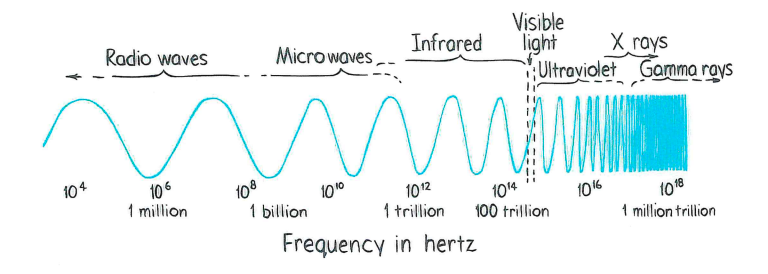
\includegraphics[width=0.8\textwidth]{fotos/visible_spectrum.png}
  \end{figure}

  \noindent According to Maxwell equations we know that time-changing electric fields generate magnetic fields in the vacuum and viceversa. The speed of this oscilating wave in vacuum is what we call $c=\frac{1}{\sqrt{\varepsilon_0\mu_0}}$
  \clearpage

  \section{A Basic Review of Simple Harmonic Motion}
    \subsection{Spring}
      \noindent Figure a massless spring. We know that springs exert a force contrary to a movement out of equilibrium. That force will be proportional to $kx$ being $k$ the spring constant. Depending on wether you push or pull on a spring you'll get a positive or a negative force. According to Newton's Second Law:
      \begin{equation}
        \vec{a}(t)=\dfrac{\vec{F}(t)}{m}
      \end{equation}
      \noindent If an object moves at a constant velocity through vacuum, it has no acceleration, but if velocity is not constant, what would that non-zero acceleration be? This question raises Newton's Second Law.\\

      \noindent When we pull from a spring with a mass attached and we leave it free, the mass will accelerate with less and less force until it arrives to the equilibrium point of the spring. At that point the force will be zero, but the mass will continue its trajectory according to the Laws of Conservation of Momentum and Energy,
      but this time the force exerted by the spring will be negative, opposing to the movement and stopping the mass at some point (The same as the start one but from the other side). This movement will continue in an oscillatory manner infinitelly. We have our Harmonic Oscillator.
      \begin{equation}
        \vec{a}(t)=\dfrac{-k}{m}\vec{x}(t)
      \end{equation}
      \noindent In our problem, we are describing a cosine function. A sinusoidal function that has some amplitude equal to the separation we initially took from the spring's equillibrium point. Velocity is the slope of position, then it is it's derivative. We can say the same about the acceleration as we can see:
      \begin{equation}
        x(t)=\cos(t)\hspace{1cm}v(t)=\dfrac{d}{dt}(\cos(t))=-\sin(t)\hspace{1cm}a(t)=\dfrac{d}{dt}(-\sin(t))=-\cos(t)
      \end{equation}
      \noindent But how do we know that is the only possible position funciton? It is not, this one only works for $k=m$ for example:
      \begin{equation}
        x(t)=\cos(2t)\hspace{1cm}v(t)=-2\sin(2t)\hspace{1cm}a(t)=-2^2\cos(2t)
      \end{equation}
      Which only works for $\dfrac{k}{m}=2^2$
      \begin{equation}
        x(t)=\cos(3t)\hspace{1cm}v(t)=-3\sin(3t)\hspace{1cm}a(t)=-3^2\cos(3t)
      \end{equation}
      Which only works for $\dfrac{k}{m}=3^2=9$\\

      \noindent We can derive by innduction that $a(t)=\dfrac{-k}{m}x(t)$ with $\omega=\sqrt{\dfrac{k}{m}}$. Then the solution would be:
      \begin{equation}
        x(t)=\cos(\omega t)
      \end{equation}

      \noindent Now we are going to think about what we call amplitude, a factor that will multiply our position function so that it "survives" the derivative and stays on our velocity and acceleration formulas.
      \begin{equation}
        x(t)=A\cos(\omega t)\hspace{1cm}v(t)=-A\omega\sin(\omega t)\hspace{1cm}a(t)=-A\omega^2\cos(\omega t)=-\omega^2 x(t)
      \end{equation}
      \noindent Which indeed satisfies the problem. We have existence, but unicity? We'll return to it in a few sections.
      \clearpage

    \subsection{What is the Physical meaning of $\omega$?}
      We claim that if $T$ is the period, then
      \begin{equation}
        T=\dfrac{2\pi}{\omega}\Longleftrightarrow\omega=\dfrac{2\pi}{T}
      \end{equation}
      But why did we assume the formula of the period to start off.
      \begin{equation}
        \cos(\omega(t+T))=\cos(\omega t)\Longleftrightarrow\cos(\omega t+\omega T)=\cos(\omega t)\Longleftrightarrow \omega T=2\pi\Longleftrightarrow T=\dfrac{2\pi}{\omega}
      \end{equation}
      \noindent In the consideration that no other force interfies to the mass, if acceleration is negatively proportional to the displacement, we have a simple harmonic movement. This is our governing, "paradigm" equation:
      \begin{equation}
        a(t)=\dfrac{d^2 x(t)}{dt^2}=-\dfrac{k}{m}x(t)=-\omega^2 x(t)\hspace{1cm}\text{with }\omega^2=\dfrac{k}{m}
        \label{eq:paradigm}
      \end{equation}
      Thus we have a set of solutions associated to the "paradigm" equation (\ref{eq:paradigm}):
      \begin{equation}
        x(t)=A\cos\left(\omega t\right)+B % Lo del B no le mola por la cara
      \end{equation}
    \section{General Sinusoidal Oscillation}
      Consider the solution of the form
      \begin{equation}
        x(t)=A\cos(\omega t +\phi)
        \label{eq:general_sinusoidal}
      \end{equation}
      For any angle $\omega$, phase constant $\phi$ and amplitude $A$, this solution satisfies the "paradigm" equation (\ref{eq:paradigm}). We know our maximum amplitude is $A$, so whenever $\cos(\omega t+\phi)=1$ we get a maximum. This happens whenever $\omega t+\phi=2\pi n$ with $n=0,1,2,\dots$ \textit{Idem.} with the minimum.\\

      \noindent We know that $\sin$ and $\cos$ are delayed by $\frac{\pi}{2}$. Then adding this phase difference to the cosine will output sinus wave. In mathematical words:
      \begin{equation}
        A\cos\left(\omega t +\phi\right)=A\sin\left(\omega t+\phi+\dfrac{\pi}{2}\right)
      \end{equation}
      Changing $\phi$ can be thought as a change in the initial conditions of our problem, on initial position and velocity at $t=0$.
      \ejemplo{Suppose that we have two identical mass-spring systems that are set into oscilaltion. Both of them oscillate at the same anglar frequency $\omega$}{
        The first mass-spring system is released at position $x+A$ at time $t=\dfrac{\pi}{2\omega}$. Then, its subsequent $x(t)$ is given by $x(t)=A\cos\left[\omega\left(t+\dfrac{\pi}{2\omega}\right)\right]$
      }
      \noindent Acceleration is not a free condition, as by equation (\ref{eq:paradigm}) if you set an initial position and velocity, then acceleration is already specified. Accordingly, if you choose an initial acceleration and velocity, your presentation is already set. Thus only two of the variables are free at the same time.
      \teorema{}{If you specify the position and the velocity of a given simple harmonic oscillator system at any time $t=t_0$, then the subsequent motion is completely and uniquely specified. (Unless an external agent later interfies with the motion).}
      \noindent Returning to the formula (\ref{eq:general_sinusoidal}) we can derive the theorem:

      \teorema{}{If you specify the position and velocity of an ideal oscillator system at the time $t=0$ then the subsequent motion is uniquely specified by the formula $x(t)=A\cos(\omega t+\phi)$ for some unique pair of constants $A$ and $\phi$.}

      \corolario{}{If $x(t=t_0)$ and $v(t=t_0)$ are specified (where $t_0\neq 0$) then $x(t)=A\cos\left[\omega(t-t_0)+\phi\right]$ for unique $\left\{A\text{ and }\phi\right\}$}
      \ejemplo{Consider, say, a mass-spring system for which, say, $k=15\frac{N}{m}$ and $m=5\ kg$. Suppose that, at $t=0$ the mass is thrown from possition $x_0=1.7\ m$ from equilibrium with velocity $v_0=+4.2\frac{m}{s}$. What is the subsequent motion?}{
        Since this is a general sinusoidal simple harmonic motion, we're going to use the formula (\ref{eq:general_sinusoidal}). WE know that we can find unique constants $A$ and $\phi$ because of the previous theorems and corollary. By definition, $\omega=\sqrt{\frac{k}{m}}=\sqrt{\frac{15}{6}}=\sqrt{3}$. Then we have $x(t)=A\cos(\sqrt{3}t+\phi)$. Now we apply our initial conditions:
        \begin{enumerate}
          \item $x(t=0)=x_0=1.7=A\cos(\sqrt{3}\cdot 0+\phi)\Longrightarrow {1.7=A\cos{\phi}}$
          \item $v(t=0)=v_0=4.2=-\sqrt{3}A\sin(\phi)\Longrightarrow{4.2=-\sqrt{3}A\sin(\phi)}$
        \end{enumerate}
        We have two equations and two unknowns, then we know algebraically that we have a existence and unicity of a solution. Dividing the second equation by the first.
        \[\dfrac{4.2}{1.7}=-\sqrt{3}\tan(\phi)\Longleftrightarrow \boxed{\phi=\arctan\left(-\dfrac{2.47}{\sqrt{3}}\right)=-0.959\ rad}\]
        Now substituting in the first equation
        \[1.7=A\cos(\phi)\Longleftrightarrow \boxed{A=\dfrac{1.7}{\cos(0.959)}=2.96}\]
        Therefore our final equation will be:
        \[\boxed{x(t)=2.96\cos(\sqrt{3}t-0.959\ rad)}\]
      }
    \clearpage
    \section{Energy in Simple Harmonic Motion}
        Imagine an electron oscilating due to a combination of fields. As we know, a moving charge will loose energy by radiation, making the amplitude decay with time. If we ignore it, the amplitude should be constant and thus the kinetic energy. 
        \begin{equation}
          K=\dfrac{1}{2}mv^2(t)
        \end{equation}
        But how does it depend on time? As we know
        \[
          x(t)=A\cos(\omega t+\varphi)\hspace{1cm}v(t)=-\omega A\sin(\omega t+\varphi)\hspace{0.5cm}\Longrightarrow\hspace{0.5cm}v^2(t)\omega^2 A^2\sin^2(\omega t+\varphi)
        \]
        \begin{equation}
          K=\dfrac{1}{2}m\omega^2 A^2\sin^2(\omega t+\varphi)\Longleftrightarrow\boxed{K=\dfrac{1}{2}\dfrac{k}{m}A^2\sin^2(\omega t+\varphi)}
        \end{equation}\hspace{0cm}\\
         
        \begin{wrapfigure}[14]{l}{0.5\textwidth}
          \vspace{-1.4cm}
          \centering
          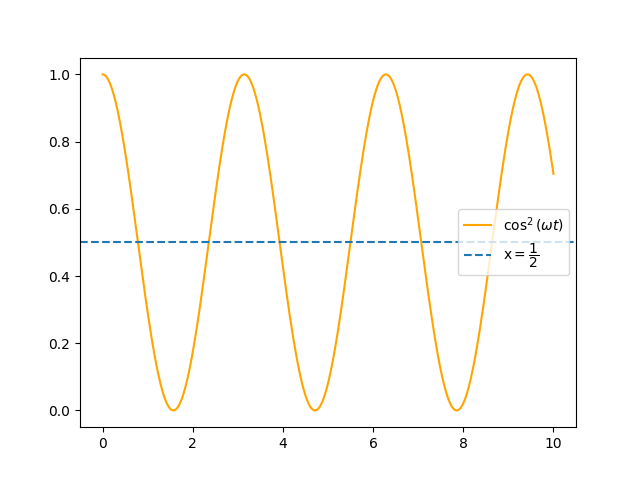
\includegraphics[width=\textwidth]{fotos/cos2.png}
        \end{wrapfigure}

        \noindent If we look at the graph of the kinetic energy, we'll observe that the period of the energy is half of what the oscillation had. So the kinetic energy is not constant. Where is the energy when the kinetic energy is zero? It must be potential.\\

        \noindent We know that the equation for the potential energy of a spring is $W=\frac{1}{2}k\Delta x$. But where does it come from?
        \begin{equation}
          stuff
        \end{equation}
        \hspace{0cm}\\\hspace{0cm}\\

        \begin{wrapfigure}[14]{l}{0.5\textwidth}
          \vspace{-1.4cm}
          \centering
          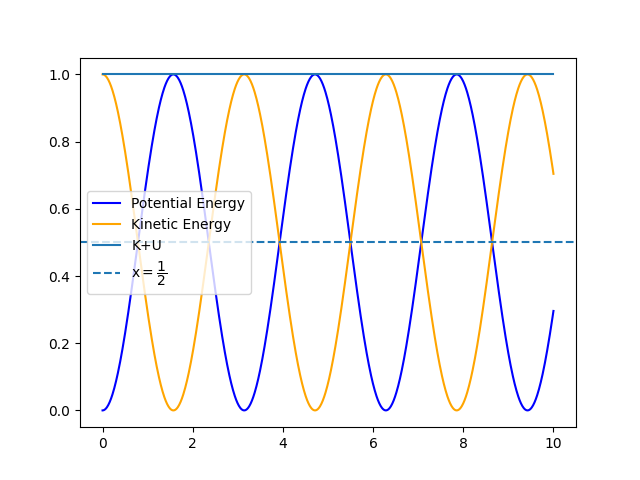
\includegraphics[width=\textwidth]{fotos/energies.png}
        \end{wrapfigure}

        \noindent If we then plot both potential and kinetic energy, we can see how they have a phase of $\nicefrac{\pi}{2}$, so that when we add up both of them, we get a constant value, and thus satisfy the conservation of energy law.
        
        \begin{equation}
          \begin{aligned}
          &K+U=\dfrac{1}{2}kA^2\sin^2(\omega t+\varphi)+\dfrac{1}{2}kA^2\cos^2(\omega t+\varphi)\\
          &K+U=\dfrac{1}{2}kA^2\left(\sin^2(\omega t+\varphi)+\cos^2(\omega t+\varphi)\right)\\
          &\boxed{E = \dfrac{1}{2}kA^2}
          \end{aligned}
        \end{equation}
        If we want to get our max possible velocity, we know that then $K$ must be at a max, so $K=E=\dfrac{1}{2}kA^2$ and solve for $v$:
        \begin{equation}
          \dfrac{1}{2}mv^2=\dfrac{1}{2}kA^2\Longleftrightarrow v_\text{max}=\sqrt{\dfrac{k}{m}}A=\omega A
        \end{equation}
        
        \clearpage
        \subsection{Time averages}
          \noindent We are usually interested on the time average of the function. 
          \definicion{Time average}{
            The time function of any function $f(t)$ is denotef by $\langle f(t)\rangle_T$ 
            \[\langle f(t)\rangle_T=\dfrac{1}{T}\int_{t_0}^{t_0+T}f(t^\prime)dt^\prime\]
          }
          \noindent So in our case we want $\langle\cos^2(\omega t+\varphi)\rangle_T$ where $T$ is one period. We'll claim that this value is $\nicefrac{1}{2}$ We can proof this by plotting $\cos^2(\omega t)$ and seeing that the oscillation is symmetrical around the value $\nicefrac{1}{2}$. Moreover you can also deduce this from the next trigonometric identity.
          \[\cos^2\theta=\dfrac{1}{2}+\dfrac{1}{2}\cos(2\theta)\Longleftrightarrow\langle\cos^2\theta\rangle_T=\langle\dfrac{1}{2}\rangle_T=\dfrac{1}{2}\]
      \section{Governing ODE}
        The mass-spring system ODE is $m x^{\prime\prime}=-k\cdot x(t)$. This is obtained from the conservation of energy's law.
        \[U(x)=\int_0^x F(x^\prime)\ dx^\prime=\int_0^x kx^\prime\ dx^\prime=\dfrac{1}{2}kx^2\]
        \[K=\dfrac{1}{2}m{x^{\prime}}^2\]
        \noindent By the previous development, we got that $K+U$ is constant, so it's time derivative should be $0$.
        \[\dfrac{d}{dt}\left(\dfrac{1}{2}m{x^\prime}^2+\dfrac{1}{2}kx^2\right)=0\Longleftrightarrow\dfrac12 m\dfrac{d}{dt}\left({x^\prime}^2\right)+\dfrac12 k\dfrac{d}{dt}(x^2)=0\Longleftrightarrow m x^\prime x^{\prime\prime}+kxx^\prime=0\Longleftrightarrow x^\prime\left(mx^{\prime\prime}+kx\right)=0\]
        So as velocity isn't zero ($x^\prime\neq0$), then the other term must be zero $\left(mx^{\prime\prime}+kx\right)=0 \Longrightarrow mx^{\prime\prime}+kx=0$
        \begin{equation}
          x^{\prime\prime}=-\dfrac{k}{m}x
        \end{equation}
      \section{Simple Pendulum}
        \begin{figure}[h!]
          pendulum
        \end{figure}
        \noindent We've got two forces, the Tension (radial force) and the Earth's force on the mass, weight (radial force). Then the mass moves tangentially, so that weight oposes tension on one component, and imposes a tangential force with the other component, introducing an oscillatory movement.
        \[F_t=-mg\sin\theta\Longleftrightarrow ms^{\prime\prime}(t)=-mg\sin(\theta(t))\]
        We'll work only on terms of theta so we convert $s=l\theta_{t_0}$ so that:
        \[\theta^{\prime\prime}(t)=-\dfrac{g}{l}\sin{\theta}(t)\]
        If we approximate the ODE for small angles, then we have a simple harmonic oscillation, from which we know the solution is
        \begin{equation}
          \theta(t)=A\cos\left(\sqrt{\dfrac{g}{l}}t+\phi\right)
        \end{equation}
      \clearpage
      \section{The LC circuits}
        \begin{itemize}
          \item The law of capacitors states that $V=\nicefrac{Q}{C}$ being C a constant for each capacitor.
          \item The law of inductors states that $\varepsilon = -L\frac{dI}{dt}$, the minus sign reflects Lenz's Law. The IEMF induced oposes the rate of change of the current intensity.
        \end{itemize}

        \noindent Capacitors and Inductors oppose in some way, because the capacitor wants to empty its charge as fast as possible, meanwhile the inductor opposes the change of intensity. Is this a shm?\\

        \noindent As the capacitor starts to discharge, the inductor starts to lessen the slope.
        \[\left|\dfrac{dI}{dt}\right|=\dfrac{V_c}{L}=\dfrac{Q}{LC}\]
        \noindent As $Q$ decreases, the slope of the intensity lessens and lessens until we reach a time where there isn't excess charge on any plate of the capacitor. At that time, the current is at it's maximum value, and it is not changing at that instant.\\

        \noindent Charges in movement are the current itself. And as moving as they are, they have momemtum that they can't dump, so the current won't stop, it will keep going, charging the capacitor with the opposite charge, overshooting. Firstly the current decreases slowly, accelerating with time.\\

        \noindent When the current achieves zero, the capacitor is fully charged with the opposite sign charge. Then it is going to keep oscillating the equilibrium. We don't know yet if this oscillating movement is shm. Let's approach it with the governing equation.
          \subsection{Governing Equation Approach}
            \noindent The behaviour is analogous to the mass spring system.
            \[\dfrac{Q}{C}=-L\dfrac{dI}{dt}\hspace{1cm}I\equiv\dfrac{dQ}{dt}\ \Longrightarrow\ \dfrac{d^2Q}{dt^2}=-\dfrac{1}{LC}Q(t)\ \text{\ which is a smh governing equation} \]
            \noindent The motion of the charghe is thus simple harmonic. The solution will be $Q=Q_0\cos\left(\nicefrac{t}{\sqrt{LC}}+\phi\right)$. As $Q(t)$ is a \textit{smh}, then $I(t)$ is one too, as $I(t)=Q^\prime(t)$. If you take the derivative of the governing equation, you end up with another \text{smh} governing equation concerning $I(t)$ instead of $Q(t)$. 
            \begin{equation}
              \boxed{\dfrac{d^2Q}{dt^2}=-\dfrac{1}{LC}Q(t)}\hspace{1cm}\boxed{\dfrac{d^2I}{dt^2}=-\dfrac{1}{LC}I(t)}
            \end{equation}
            \noindent But we know that they are not in phase with each other. That happens because $I(t)=Q^\prime (t)$, and thus if one is sinusoidal, the other will be cosenoidal and viceversa. Same happens with the amplitude, you take the $Q_\text{max}$ out of the equation when you derive, making the intensity amplitude different. $I_\text{max}=\omega Q_\text{max}$ with $\omega=\nicefrac{1}{\sqrt{LC}}$\\

            \noindent If we see the mass as the resistance to changes in acceleration, we can see the simillarity with the inductance, which resists changes in current intensity. With the same logic, we can see how $Q$ is analogous to $x$ and $I$ is analogous to $v$.
          \subsection{Energy Approach}
            \noindent We can recall the enenrgy between the plates of a capacitor:
            \[U_E=\dfrac{1}{2}\dfrac{Q^2}{C}=\dfrac12\varepsilon_0 E^2\cdot \text{ volume between the capacitor plates}\]
            \[Q(t)=Q_\text{max}\cos(\omega t+\phi)\Longrightarrow U_E=\dfrac{1}{2C}Q^2_\text{max}\cos^2(\omega t+\phi)\]
            \noindent It is analogous too in the potential energy on the mass spring system. If we take a look at the energy stored at the inductor:
            \[U_B=\dfrac{1}{2}LI^2=\dfrac{B^2}{2\mu_0}\cdot \text{ volume enclosed by the inductor}\]
            \[Q(t)=Q_\text{max}\cos(\omega t+\phi)\Longrightarrow U_B=\dfrac{1}{2}LI^2_\text{max}\sin^2(\omega t+\phi)\]
            \noindent Which is now analogous to the kinetic energy.\\

            \noindent Both energies oscilates in time. But they don't do it in phase as one is a sinus and the other a cosinus. There is a phase shift. The total energy is
            \begin{equation}
             \boxed{ U=\dfrac{Q_\text{max}^2}{2C}=cte}
            \end{equation}
            \noindent The system produces radiation, which resistance is analogous to the air resistance in the mass-spring system.
      \section{Plasma Oscillations (K.2.22-K.2.23)}
        \noindent Plasma is matter where electrons are separated from the atomic/mollecular cores. There's plasma in Earth's atmosphere, the solar corona, interstellar gas, fluorescent lamps... \\

        \noindent If we think of a box filled with $N$ electrons per $m^3$ neutralized by positive ions. We generate an electric field constant in a determined direction and suddenly turn it off. Thus the plasma polarizes, while the electric field has not gone away we have essentially two fields, one from the field we set up initially, and one that oposes the first field, because on the extremes of the area charges would exit and unalign the plasma. When the first electric field is removed, the oposing field remains.\\

        \noindent The plasma is by no means static, but we can say that the mean speed will be consntant at zero because the electrons are moving in a random manner. Thus the average electron motion is zero. The only movement that will be seen is that generated by the electric field we imposed in the medium. We'll call the external field $\vec{E}_{\text{ext}}=E_\text{ext}\hat{x}$. The system is analogous to a plasma medium between two capacitor plates which are removed after a certain time.\\

        \noindent In the plasma, the compensating electric field is given by 
        \[E=\dfrac{\sigma}{E_0}\hspace{1cm}\text{Where }\sigma \text{ is the generated effective surface charge density }\sigma=ne\Delta x\]
        \noindent Then the field should be
        \[\vec{E}_\text{comp}=\dfrac{+ne}{\varepsilon_0}\hat{x}\]
        \noindent We are now going to try and find our governing differential equation:
        \begin{equation}
          m_e\dfrac{d^2x(t)}{dt^2}=-\dfrac{ne^2}{\varepsilon_0}x(t)
        \end{equation}
        \noindent It's equivilbiurm angelar frequency "Plasma Frequency" would then be:
        \begin{equation}
          \omega_p=\sqrt{\dfrac{ne^2}{m_e\epsilon_0}}\ \left[\dfrac{\text{rad}}{s}\right] \Longleftrightarrow f_p=\dfrac{\omega_p}{2\pi}=\sqrt{\dfrac{e^2}{4\pi^2 m_e\varepsilon_0}}\sqrt{n}
        \end{equation}
        \noindent We will ignore loss of energy due to electromagnetic radiantion from the oscillating, accelerating electrons, and from the collision of particles.\\

        \noindent Faltan la segunda parte de la clase pero me ha dado pereza
        \clearpage
      \section{The "Quick Energy Method"}
        \noindent As a notation we'll introduce $q(t)\equiv\psi(t)$ 
        \teorema{Quick Energy Theorem}{
          If tthe total energy of oscillation (kinetic + potential) can be written in the form
          \begin{equation}
            E=a\dot{q}^2 + bq^2+c
          \end{equation}
          Where $a$ and $b$ are positive constants, then $q$ undergoes simple harmonic motion with angular frequency 
          \begin{equation}
            \omega=\sqrt{\dfrac{b}{a}}
          \end{equation}
        }
        \subsubsection*{Proof}
        \[E=a\dot{q}^2+bq^2+c\Longleftrightarrow 0=\dfrac{dE}{dt}=2a\dot{q}\ddot{q}+2bq\dot{q}\Longleftrightarrow 2\dot{q}\left(a\ddot{q}+bq\right)\Longleftrightarrow a\ddot{q}+bq=0\Longleftrightarrow\boxed{\ddot{q}=-\dfrac{b}{a}q}\]
        \hspace{1.2cm}Which is our governing equation from which we have plenty of knowledge to affirm that $\omega=\sqrt{\nicefrac{b}{a}}$\\

        \noindent If the energy is not separately quadratic in $q$ and $\dot{q}$, then the motion will not be simple harmonic. Although in many situations the energy can be approximated by an expression that is quadratic in $q$ and $\dot{q}$ as it happens with the pendulum. This approximating method is called \textbf{Linearization}.\\

        \noindent If we change the point of view we get a different governing differential equation. Depending on where we put the coordinate system, the ode will have a different form.\\

        \noindent This method can't be applied to anything that is not a single spring system, as a multiple mass on a spring system would not work. You would be working with the center of mass, and it is just not moving, so you would get a $0=0$.\\

      \section{The Energy Method}
          \noindent Consider two equal masses on the extremes of a spring. Energetically, we have:
          \[E=2\dfrac{1}{2}mv^2+\dfrac12 k(2k)^2=mv^2+2k\psi^2\]
          \noindent Being $2\psi$ the total stretch and $v$ the speed of either mass (equal and opposite). So:
          \[0=\dfrac{dE}{dt}=2mv\dot{v}+4k\psi\dot{\psi}\]
          \noindent Since $\dot{\psi}=v$ and $\dot{v}=\ddot{\psi}$
          \[m\dot{\psi}\ddot{\psi}+2k\psi\dot{\psi}=0\Longleftrightarrow\ddot{\psi}=\dfrac{-2k}{m}\psi\Longleftrightarrow\boxed{\omega=\sqrt{\dfrac{2k}{m}}}\]
          \noindent However, let's now suppose the masses are not equal. Consider one of them has mass $m$ and the other one has mass $2m$. The mass with less mass will stretch twice as further as the bigger one. Thus, the total stretch will be $3\psi$.
          \[m(-2\psi)^{\prime\prime}=+k(3\psi)\Longleftrightarrow 2m\ddot{\psi}=-3k\psi\Longleftrightarrow\ddot{\psi}(t)=\dfrac{-3k}{2m}\psi(t)\Longleftrightarrow\boxed{\omega=\sqrt{\dfrac{3k}{2m}}}\]
        \comentario{The reduced mass method [...]}
      \section{One mass two spring system K3.2-Kexample3.6}
          \noindent Imagine a system with two springs attached to a mass that forming a triangle [needs figure]. The mass will oscilate from the equilibrium point, at which the springs are not compressed into resting elogation $s_0$. We are going to check if this movement is simple harmonic motion. The return force is
          \[\dfrac{\text{Return Force}}{\text{mass}\cdot\text{disp}} = \dfrac{-2k(s-s_0)\sin\theta}{mx}\]
          \noindent We have three dynamic variables but we need it to be only one, so we will write everything in terms of $x$. We will use that $\sin\theta=\dfrac{x}{s}$ and $s=\sqrt{s_e^2+x^2}$ then:
          \[\dfrac{\text{Return Force}}{\text{mass}\cdot\text{disp}} = \dfrac{-2k}{m}\left(1-\dfrac{s_0}{\sqrt{s_e^2+x^2}}\right)\]
          \noindent This acceleration is not negatively proportional to the displacement, so we can state that this is not simple harmonic motion. We must do an approximation to work with this system the way we've talked before. If the oscillations are very small, then $x$ is very close to zero and the before expression is constant. When the oscillations are smaller, the system approximates more to a simple harmonic oscillator. In other words, the governing ODE:
          \[m\ddot{x}=-2k(s-s_0)\sin\theta\Longleftrightarrow m\ddot{x}=-2kx\left(1-\dfrac{s_0}{\sqrt{s_e^2+x^2}}\right)\Longleftrightarrow \ddot{x}=-\dfrac{2k}{m}\left(1-\dfrac{s_0}{s_e}\right)x\Longleftrightarrow\boxed{\omega=\sqrt{\dfrac{2k}{m}\left(1-\dfrac{s_0}{s_e}\right)}}\]
          

\end{document}
